\documentclass[a4paper]{article}
\usepackage{listings}
\usepackage{xcolor}
\definecolor{codegreen}{rgb}{0,0.6,0}
\definecolor{codegray}{rgb}{0.5,0.5,0.5}
\definecolor{codepurple}{rgb}{0.58,0,0.82}
\definecolor{backcolour}{rgb}{0.95,0.95,0.92}

\lstdefinestyle{mystyle}{
    backgroundcolor=\color{backcolour},   
    commentstyle=\color{codegreen},
    keywordstyle=\color{magenta},
    numberstyle=\tiny\color{codegray},
    stringstyle=\color{codepurple},
    basicstyle=\ttfamily\footnotesize,
    breakatwhitespace=false,         
    breaklines=true,                 
    captionpos=b,                    
    keepspaces=true,                 
    numbers=left,                    
    numbersep=5pt,                  
    showspaces=false,                
    showstringspaces=false,
    showtabs=false,                  
    tabsize=2
}

\lstset{style=mystyle}

\usepackage{tikz}
\usetikzlibrary{matrix}
\begin{document}

\section*{Python code to generate binomial trees}
The code to generate the tree is:
\begin{lstlisting}[language=Python, caption={Python extract}, extendedchars=true]
def make_binomial_tree(number_of_periods: int)-> str:
    """ Generate the Latex code to print a binomial tree
    of 'number_of_periods' periods.
    Parameters:
    number_of_periods: integer
    return string
    """
    columns = {}
    columns2 = {}
    ...
\end{lstlisting}
Please refer to the file \textit{binomial\_tree.py} for the full code.
Examples of binomial trees generated with the code for:
\subsection*{4 periods}
print(make\_binomial\_tree(4))

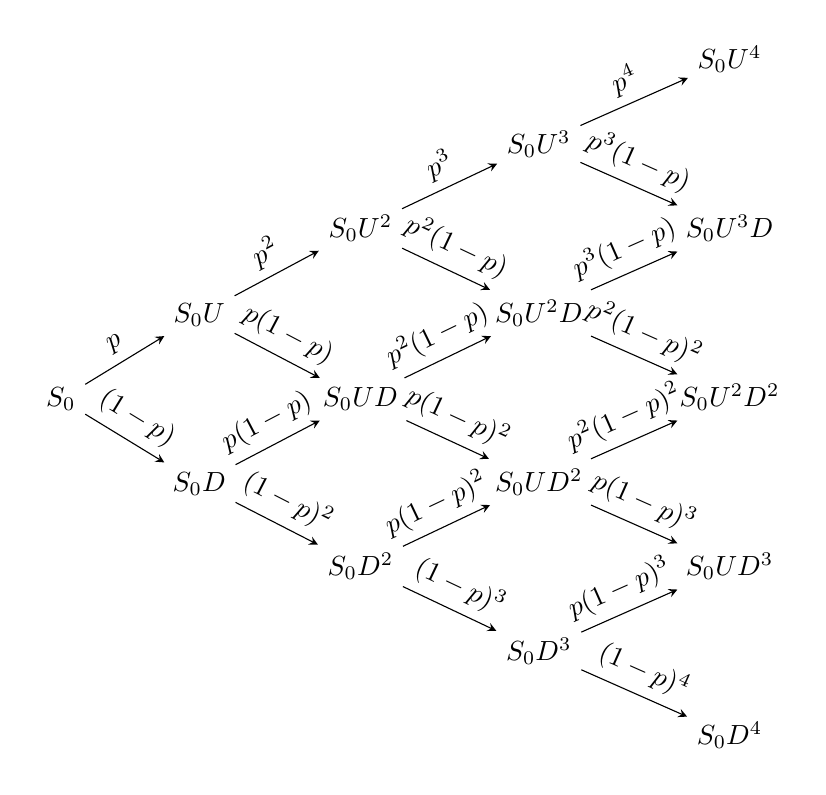
\begin{tikzpicture}[>=stealth,sloped]
            \matrix (tree) [%
            matrix of nodes,minimum size=0.5cm,
        column sep=1cm,
        row sep=0.5cm,]{ &  &  &  & $S_0U^4 $ \\
 &  &  & $S_0U^3 $ &  \\
 &  & $S_0U^2 $ &  & $S_0U^3 D$ \\
 & $S_0U $ &  & $S_0U^2 D$ &  \\
$S_0$ &  & $S_0U D$ &  & $S_0U^2 D^2$ \\
 & $S_0 D$ &  & $S_0U D^2$ &  \\
 &  & $S_0 D^2$ &  & $S_0U D^3$ \\
 &  &  & $S_0 D^3$ &  \\
 &  &  &  & $S_0 D^4$ \\
};
\draw[->] (tree-2-4) -- (tree-1-5) node [midway,above] {$ p^4  $};
\draw[->] (tree-2-4) -- (tree-3-5) node [midway,above] {$ p^3 (1-p) $};
\draw[->] (tree-3-3) -- (tree-2-4) node [midway,above] {$ p^3  $};
\draw[->] (tree-3-3) -- (tree-4-4) node [midway,above] {$ p^2 (1-p) $};
\draw[->] (tree-4-2) -- (tree-3-3) node [midway,above] {$ p^2  $};
\draw[->] (tree-4-2) -- (tree-5-3) node [midway,above] {$ p (1-p) $};
\draw[->] (tree-4-4) -- (tree-3-5) node [midway,above] {$ p^3 (1-p) $};
\draw[->] (tree-4-4) -- (tree-5-5) node [midway,above] {$ p^2 (1-p)^2 $};
\draw[->] (tree-5-1) -- (tree-4-2) node [midway,above] {$ p  $};
\draw[->] (tree-5-1) -- (tree-6-2) node [midway,above] {$  (1-p) $};
\draw[->] (tree-5-3) -- (tree-4-4) node [midway,above] {$ p^2 (1-p) $};
\draw[->] (tree-5-3) -- (tree-6-4) node [midway,above] {$ p (1-p)^2 $};
\draw[->] (tree-6-2) -- (tree-5-3) node [midway,above] {$ p (1-p) $};
\draw[->] (tree-6-2) -- (tree-7-3) node [midway,above] {$  (1-p)^2 $};
\draw[->] (tree-6-4) -- (tree-5-5) node [midway,above] {$ p^2 (1-p)^2 $};
\draw[->] (tree-6-4) -- (tree-7-5) node [midway,above] {$ p (1-p)^3 $};
\draw[->] (tree-7-3) -- (tree-6-4) node [midway,above] {$ p (1-p)^2 $};
\draw[->] (tree-7-3) -- (tree-8-4) node [midway,above] {$  (1-p)^3 $};
\draw[->] (tree-8-4) -- (tree-7-5) node [midway,above] {$ p (1-p)^3 $};
\draw[->] (tree-8-4) -- (tree-9-5) node [midway,above] {$  (1-p)^4 $};
\end{tikzpicture}
\newpage
\subsection*{3 periods}
print(make\_binomial\_tree(3))

\begin{tikzpicture}[>=stealth,sloped]
            \matrix (tree) [%
            matrix of nodes,
            minimum size=1cm,
            column sep=3.5cm,
            row sep=1cm,
            ]
        { &  &  & $S_0U^3 $ \\
 &  & $S_0U^2 $ &  \\
 & $S_0U $ &  & $S_0U^2 D$ \\
$S_0$ &  & $S_0U D$ &  \\
 & $S_0 D$ &  & $S_0U D^2$ \\
 &  & $S_0 D^2$ &  \\
 &  &  & $S_0 D^3$ \\
};
\draw[->] (tree-2-3) -- (tree-1-4) node [midway,above] {$ p^3  $};
\draw[->] (tree-2-3) -- (tree-3-4) node [midway,above] {$ p^2 (1-p) $};
\draw[->] (tree-3-2) -- (tree-2-3) node [midway,above] {$ p^2  $};
\draw[->] (tree-3-2) -- (tree-4-3) node [midway,above] {$ p (1-p) $};
\draw[->] (tree-4-1) -- (tree-3-2) node [midway,above] {$ p  $};
\draw[->] (tree-4-1) -- (tree-5-2) node [midway,above] {$  (1-p) $};
\draw[->] (tree-4-3) -- (tree-3-4) node [midway,above] {$ p^2 (1-p) $};
\draw[->] (tree-4-3) -- (tree-5-4) node [midway,above] {$ p (1-p)^2 $};
\draw[->] (tree-5-2) -- (tree-4-3) node [midway,above] {$ p (1-p) $};
\draw[->] (tree-5-2) -- (tree-6-3) node [midway,above] {$  (1-p)^2 $};
\draw[->] (tree-6-3) -- (tree-5-4) node [midway,above] {$ p (1-p)^2 $};
\draw[->] (tree-6-3) -- (tree-7-4) node [midway,above] {$  (1-p)^3 $};
\end{tikzpicture}
\newpage
\subsection*{5 periods}
print(make\_binomial\_tree(5))

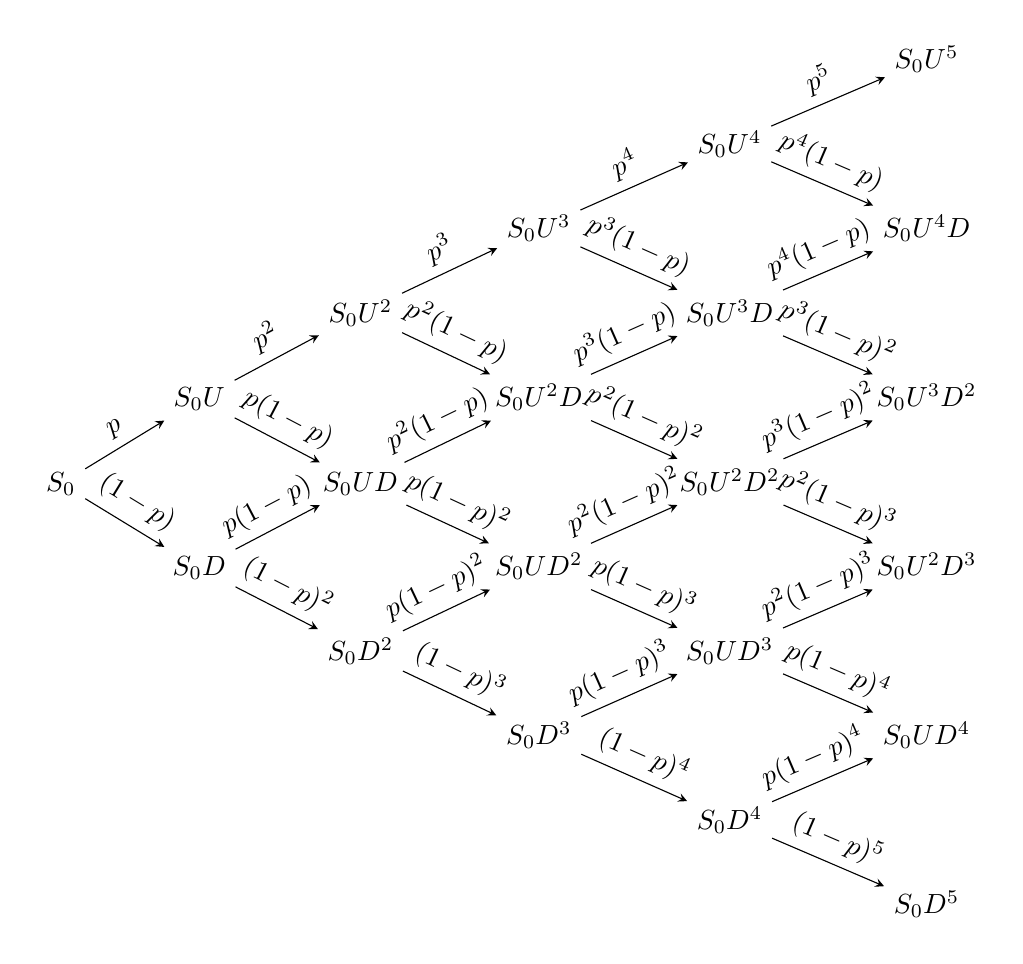
\begin{tikzpicture}[>=stealth,sloped]
            \matrix (tree) [%
            matrix of nodes,minimum size=0.5cm,
        column sep=1cm,
        row sep=0.5cm,]{ &  &  &  &  & $S_0U^5 $ \\
 &  &  &  & $S_0U^4 $ &  \\
 &  &  & $S_0U^3 $ &  & $S_0U^4 D$ \\
 &  & $S_0U^2 $ &  & $S_0U^3 D$ &  \\
 & $S_0U $ &  & $S_0U^2 D$ &  & $S_0U^3 D^2$ \\
$S_0$ &  & $S_0U D$ &  & $S_0U^2 D^2$ &  \\
 & $S_0 D$ &  & $S_0U D^2$ &  & $S_0U^2 D^3$ \\
 &  & $S_0 D^2$ &  & $S_0U D^3$ &  \\
 &  &  & $S_0 D^3$ &  & $S_0U D^4$ \\
 &  &  &  & $S_0 D^4$ &  \\
 &  &  &  &  & $S_0 D^5$ \\
};
\draw[->] (tree-2-5) -- (tree-1-6) node [midway,above] {$ p^5  $};
\draw[->] (tree-2-5) -- (tree-3-6) node [midway,above] {$ p^4 (1-p) $};
\draw[->] (tree-3-4) -- (tree-2-5) node [midway,above] {$ p^4  $};
\draw[->] (tree-3-4) -- (tree-4-5) node [midway,above] {$ p^3 (1-p) $};
\draw[->] (tree-4-3) -- (tree-3-4) node [midway,above] {$ p^3  $};
\draw[->] (tree-4-3) -- (tree-5-4) node [midway,above] {$ p^2 (1-p) $};
\draw[->] (tree-4-5) -- (tree-3-6) node [midway,above] {$ p^4 (1-p) $};
\draw[->] (tree-4-5) -- (tree-5-6) node [midway,above] {$ p^3 (1-p)^2 $};
\draw[->] (tree-5-2) -- (tree-4-3) node [midway,above] {$ p^2  $};
\draw[->] (tree-5-2) -- (tree-6-3) node [midway,above] {$ p (1-p) $};
\draw[->] (tree-5-4) -- (tree-4-5) node [midway,above] {$ p^3 (1-p) $};
\draw[->] (tree-5-4) -- (tree-6-5) node [midway,above] {$ p^2 (1-p)^2 $};
\draw[->] (tree-6-1) -- (tree-5-2) node [midway,above] {$ p  $};
\draw[->] (tree-6-1) -- (tree-7-2) node [midway,above] {$  (1-p) $};
\draw[->] (tree-6-3) -- (tree-5-4) node [midway,above] {$ p^2 (1-p) $};
\draw[->] (tree-6-3) -- (tree-7-4) node [midway,above] {$ p (1-p)^2 $};
\draw[->] (tree-6-5) -- (tree-5-6) node [midway,above] {$ p^3 (1-p)^2 $};
\draw[->] (tree-6-5) -- (tree-7-6) node [midway,above] {$ p^2 (1-p)^3 $};
\draw[->] (tree-7-2) -- (tree-6-3) node [midway,above] {$ p (1-p) $};
\draw[->] (tree-7-2) -- (tree-8-3) node [midway,above] {$  (1-p)^2 $};
\draw[->] (tree-7-4) -- (tree-6-5) node [midway,above] {$ p^2 (1-p)^2 $};
\draw[->] (tree-7-4) -- (tree-8-5) node [midway,above] {$ p (1-p)^3 $};
\draw[->] (tree-8-3) -- (tree-7-4) node [midway,above] {$ p (1-p)^2 $};
\draw[->] (tree-8-3) -- (tree-9-4) node [midway,above] {$  (1-p)^3 $};
\draw[->] (tree-8-5) -- (tree-7-6) node [midway,above] {$ p^2 (1-p)^3 $};
\draw[->] (tree-8-5) -- (tree-9-6) node [midway,above] {$ p (1-p)^4 $};
\draw[->] (tree-9-4) -- (tree-8-5) node [midway,above] {$ p (1-p)^3 $};
\draw[->] (tree-9-4) -- (tree-10-5) node [midway,above] {$  (1-p)^4 $};
\draw[->] (tree-10-5) -- (tree-9-6) node [midway,above] {$ p (1-p)^4 $};
\draw[->] (tree-10-5) -- (tree-11-6) node [midway,above] {$  (1-p)^5 $};
\end{tikzpicture}
\end{document} 